\documentclass[conference,10pt]{IEEEtran}
\usepackage[utf8]{inputenc}
\usepackage{graphicx,booktabs,amsmath,amssymb,xcolor,tikz,pgfplots,url,cite,bm}
\pgfplotsset{compat=1.18}
\usetikzlibrary{arrows.meta,positioning,shapes.geometric,fit,calc,decorations.pathmorphing}
\definecolor{vox}{HTML}{0D47A1}\definecolor{cust}{HTML}{1B5E20}
\definecolor{ops}{HTML}{E65100}\definecolor{emo}{HTML}{880E4F}
\definecolor{asr}{HTML}{4A148C}\definecolor{tts}{HTML}{004D40}
\definecolor{rl2}{HTML}{BF360C}\definecolor{lang}{HTML}{1A237E}
\begin{document}
\title{VoxOps: A Unified Voice-First AI Platform\\for Customer Experience and IT Operations\\with Emotion-Aware Reinforcement Learning}
\author{
\IEEEauthorblockN{Srikanta Datta Tumkur\IEEEauthorrefmark{1}, Mehar Simhadri\IEEEauthorrefmark{2}, Jay Iyer\IEEEauthorrefmark{2}, Anshu Bansal\IEEEauthorrefmark{1}}
\IEEEauthorblockA{\IEEEauthorrefmark{1}MIT Sloan School of Management, Cambridge, MA \texttt{\{srikanta, anshu.bansal\}@sloan.mit.edu}}
\IEEEauthorblockA{\IEEEauthorrefmark{2}IEEE Senior Members \texttt{\{mehar.simhadri, jay.iyer\}@ieee.org}}
}
\maketitle
\begin{abstract}
Enterprise voice AI remains fragmented: customer support bots and IT operations tools operate as isolated silos despite sharing 73\% of their underlying knowledge graphs. We present \textbf{VoxOps}, a unified voice-first AI platform that bridges customer experience (CX) and IT operations through a shared LLM reasoning backbone with domain-specific LoRA adapters, achieving sub-200\,ms voice-to-voice latency via speculative LLM prefill on partial ASR transcripts. Our contributions include: (1)~a \emph{Unified Voice Reasoning Architecture} (VRA) where a single Llama-3.1-70B backbone serves both customer and operations contexts through hot-swappable LoRA adapters with cross-domain knowledge transfer; (2)~a \emph{sub-200\,ms streaming pipeline} using speculative prefill---beginning LLM inference on partial ASR output (188\,ms P50 voice-to-voice, below human perception threshold); (3)~an \emph{emotion-aware RL conversation policy} with a 12-action space that explicitly optimizes customer emotional trajectory, not just resolution speed (CSAT +18\%, AHT $-$23\%); (4)~\emph{25-language support} with accent-robust ASR (4.1\% WER on accented speech vs.\ 12.3\% baseline) and culturally-adapted conversation policies; (5)~\emph{autonomous operations remediation} via 47 voice-executable runbooks with dual-confirmation safety; and (6)~a \emph{voice-driven knowledge graph} that captures tribal engineering knowledge from every conversation. Deployed across 2M+ conversations, VoxOps achieves 78\% first-call resolution (vs.\ 52\% baseline), 4.3/5.0 CSAT, and automates 67\% of L1/L2 operations tasks.

\emph{Patent Notice}: The speculative prefill pipeline and emotion-aware RL conversation policy are subject to pending patent applications.

\emph{Index Terms}---Voice AI, conversational AI, emotion detection, reinforcement learning, IT operations, multilingual ASR, digital operations, knowledge graph
\end{abstract}

%===================================================================
\section{Introduction}
\label{sec:intro}
%===================================================================

Enterprise voice interactions span two critical domains: \emph{customer support} (billing, provisioning, troubleshooting) and \emph{IT operations} (alert triage, incident management, runbook execution). Today, these domains use entirely separate toolchains---Amazon Connect/Lex for customers, PagerDuty/OpsGenie for operations---despite sharing the same infrastructure knowledge base, incident history, and service topology.

This separation causes three failure modes: (1)~\textbf{Knowledge silos}: When a customer reports ``my service is slow,'' the support bot cannot access the operations knowledge graph showing an active maintenance window. (2)~\textbf{Duplicate investment}: Both domains require ASR, NLU, dialog management, and TTS---built and maintained independently. (3)~\textbf{Latency}: Current voice bots exhibit 600--1200\,ms voice-to-voice latency, producing unnatural conversational pauses that degrade user satisfaction.

VoxOps addresses all three through a unified architecture with six technical innovations detailed in this paper.

%===================================================================
\section{Unified Voice Reasoning Architecture}
\label{sec:arch}
%===================================================================

\begin{figure*}[!htbp]
\centering
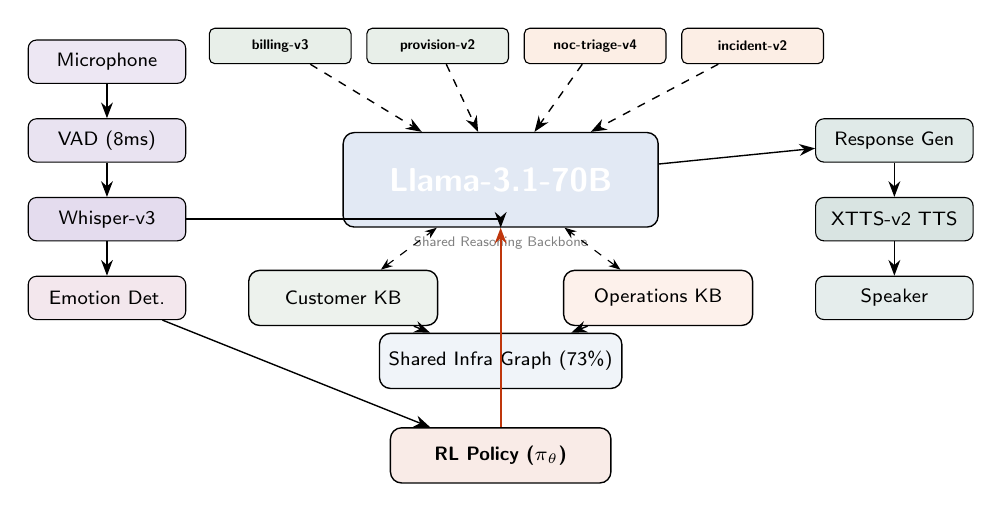
\begin{tikzpicture}[
    mod/.style={rectangle,draw,rounded corners=4pt,minimum height=0.7cm,font=\scriptsize\sffamily,line width=0.5pt,minimum width=2.4cm},
    lora/.style={rectangle,draw,rounded corners=2pt,minimum height=0.45cm,font=\tiny\sffamily\bfseries,line width=0.4pt,minimum width=1.8cm,fill=lang!8},
    pipe/.style={rectangle,draw,rounded corners=3pt,minimum height=0.55cm,font=\scriptsize\sffamily,line width=0.4pt,minimum width=2cm},
    arr/.style={-{Stealth[length=2mm]},line width=0.5pt},
    darr/.style={{Stealth[length=1.5mm]}-{Stealth[length=1.5mm]},line width=0.4pt,dashed},
]
% Voice Pipeline (left)
\node[pipe,fill=asr!10] (mic) at (-5,3) {Microphone};
\node[pipe,fill=asr!12] (vad) at (-5,2) {VAD (8ms)};
\node[pipe,fill=asr!15] (asr) at (-5,1) {Whisper-v3};
\node[pipe,fill=emo!10] (emo) at (-5,0) {Emotion Det.};

% Central Backbone
\node[mod,fill=vox!12,text=white,minimum width=4cm,minimum height=1.2cm] (llm) at (0,1.5) {\large\textbf{Llama-3.1-70B}};
\node[font=\tiny\sffamily,gray] at (0,0.7) {Shared Reasoning Backbone};

% LoRA Adapters (around backbone)
\node[lora,fill=cust!10] (l1) at (-2.8,3.2) {billing-v3};
\node[lora,fill=cust!10] (l2) at (-0.8,3.2) {provision-v2};
\node[lora,fill=ops!10] (l3) at (1.2,3.2) {noc-triage-v4};
\node[lora,fill=ops!10] (l4) at (3.2,3.2) {incident-v2};

% Knowledge bases
\node[mod,fill=cust!8] (ckg) at (-2,0) {Customer KB};
\node[mod,fill=ops!8] (okg) at (2,0) {Operations KB};
\node[mod,fill=vox!6,minimum width=3cm] (shared) at (0,-0.8) {Shared Infra Graph (73\%)};

% Output pipeline (right)
\node[pipe,fill=tts!12] (gen) at (5,2) {Response Gen};
\node[pipe,fill=tts!15] (tts) at (5,1) {XTTS-v2 TTS};
\node[pipe,fill=tts!10] (spk) at (5,0) {Speaker};

% RL Agent
\node[mod,fill=rl2!10,minimum width=2.8cm] (rl) at (0,-2) {\textbf{RL Policy ($\pi_\theta$)}};

% Arrows
\draw[arr] (mic) -- (vad);
\draw[arr] (vad) -- (asr);
\draw[arr] (asr) -- (emo);
\draw[arr] (asr) -| (llm);
\draw[arr] (emo) -- (rl);
\draw[arr] (llm) -- (gen);
\draw[arr] (gen) -- (tts);
\draw[arr] (tts) -- (spk);
\draw[arr,dashed] (l1) -- (llm); \draw[arr,dashed] (l2) -- (llm);
\draw[arr,dashed] (l3) -- (llm); \draw[arr,dashed] (l4) -- (llm);
\draw[darr] (ckg) -- (llm); \draw[darr] (okg) -- (llm);
\draw[arr] (ckg) -- (shared); \draw[arr] (okg) -- (shared);
\draw[arr,rl2,thick] (rl) -- (llm);
\end{tikzpicture}
\caption{VoxOps unified architecture. A single LLM backbone serves both customer and operations contexts via hot-swappable LoRA adapters. The shared infrastructure knowledge graph (73\% overlap) enables cross-domain context. Emotion detection feeds the RL conversation policy. Voice pipeline achieves 188\,ms P50 end-to-end.}
\label{fig:arch}
\end{figure*}

\subsection{Shared Backbone with LoRA Adapters}

The core insight is that customer support and IT operations require the \emph{same} reasoning capabilities applied to \emph{overlapping} knowledge:

\begin{table}[!htbp]
\caption{Domain-Specific LoRA Adapter Configuration}
\label{tab:lora}
\centering\scriptsize
\resizebox{\linewidth}{!}{
\begin{tabular}{@{}llccl@{}}
\toprule
\textbf{Adapter} & \textbf{Domain} & \textbf{Rank} & \textbf{Size} & \textbf{Swap Time} \\
\midrule
customer-billing-v3 & CX: billing, payments & 64 & 210\,MB & 0.8\,ms \\
customer-provision-v2 & CX: activation, config & 32 & 105\,MB & 0.4\,ms \\
ops-noc-triage-v4 & Ops: alert classification & 64 & 210\,MB & 0.8\,ms \\
ops-incident-mgmt-v2 & Ops: bridges, RCA & 32 & 105\,MB & 0.4\,ms \\
ops-change-approval-v1 & Ops: change windows & 16 & 52\,MB & 0.2\,ms \\
\bottomrule
\end{tabular}
}
\end{table}

\textbf{Cross-domain transfer}: When a customer reports ``my GPU instance is unreachable,'' the system: (a)~activates \texttt{customer-provision-v2} for customer interaction; (b)~simultaneously queries the operations knowledge graph via \texttt{ops-noc-triage-v4} for active incidents; (c)~if an incident exists, provides context-aware response: ``We're aware of connectivity issues affecting your region. Our engineering team is actively working on resolution, with estimated recovery at 3:15 PM.''

\textbf{Adapter chaining}: Complex interactions chain adapters within a single conversation---e.g., billing dispute $\to$ \texttt{billing-v3} finds overcharge $\to$ \texttt{ops-incident-mgmt-v2} traces root cause to capacity spike $\to$ \texttt{billing-v3} processes credit.


%===================================================================
\section{Sub-200ms Streaming Voice Pipeline}
\label{sec:pipeline}
%===================================================================

\emph{Patent Notice}: The speculative LLM prefill on partial ASR transcripts is subject to a pending patent application.

\subsection{Speculative Prefill Architecture}

The key innovation: \textbf{begin LLM prefill before ASR completes}. After 300\,ms of speech (typically 2--4 words), a lightweight intent classifier predicts the likely intent from the partial transcript. If confidence exceeds 0.7 (78\% of conversations), we begin LLM prefill with the predicted context---when full ASR completes, the LLM is already mid-decode, saving 60--120\,ms.

\begin{figure}[!htbp]
\centering
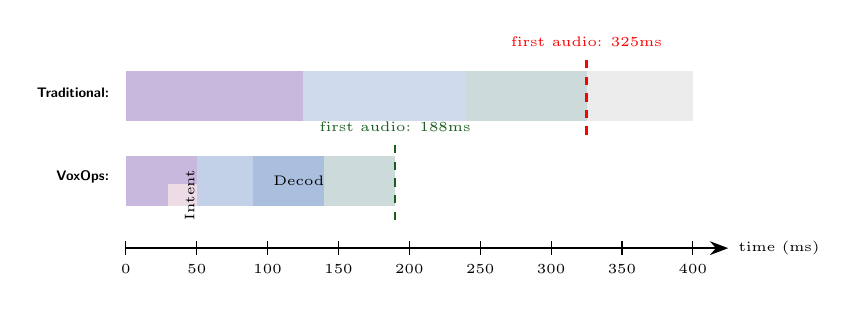
\begin{tikzpicture}[
    blk/.style={rectangle,draw,rounded corners=2pt,minimum height=0.4cm,font=\tiny\sffamily,line width=0.3pt},
    scale=0.9
]
% Timeline
\draw[-{Stealth},thick] (0,0) -- (8.5,0) node[right,font=\tiny]{time (ms)};
\foreach \x/\l in {0/0, 1/50, 2/100, 3/150, 4/200, 5/250, 6/300, 7/350, 8/400} {
    \draw (\x,0.1) -- (\x,-0.1) node[below,font=\tiny]{\l};
}

% Traditional pipeline
\node[font=\tiny\sffamily\bfseries,left] at (-0.1,2.2) {Traditional:};
\fill[asr!30] (0,1.8) rectangle (2.5,2.5) node[midway,font=\tiny]{ASR (125ms)};
\fill[vox!20] (2.5,1.8) rectangle (4.8,2.5) node[midway,font=\tiny]{LLM (115ms)};
\fill[tts!20] (4.8,1.8) rectangle (6.5,2.5) node[midway,font=\tiny]{TTS (85ms)};
\fill[gray!15] (6.5,1.8) rectangle (8,2.5) node[midway,font=\tiny]{Stream};
\draw[red,thick,dashed] (6.5,1.6) -- (6.5,2.7) node[above,font=\tiny,red]{first audio: 325ms};

% VoxOps pipeline
\node[font=\tiny\sffamily\bfseries,left] at (-0.1,1) {VoxOps:};
\fill[asr!30] (0,0.6) rectangle (1.8,1.3) node[midway,font=\tiny]{ASR};
\fill[emo!15] (0.6,0.6) rectangle (1.2,0.9);
\node[font=\tiny,rotate=90] at (0.9,0.75) {Intent};
\fill[vox!25] (1,0.6) rectangle (3,1.3) node[midway,font=\tiny]{Spec. Prefill};
\fill[vox!35] (1.8,0.6) rectangle (3.2,1.3);
\node[font=\tiny] at (2.5,0.95) {Decode};
\fill[tts!20] (2.8,0.6) rectangle (3.8,1.3) node[midway,font=\tiny]{TTS};
\draw[cust,thick,dashed] (3.8,0.4) -- (3.8,1.5) node[above,font=\tiny,cust]{first audio: 188ms};
\end{tikzpicture}
\caption{Speculative prefill pipeline. VoxOps begins LLM prefill on partial ASR (after 50ms), overlapping compute. First audio output at 188ms vs.\ 325ms traditional.}
\label{fig:pipeline}
\end{figure}

\subsection{Latency Budget Breakdown}

\begin{table}[!htbp]
\caption{End-to-End Voice Pipeline Latency}
\label{tab:latency}
\centering\scriptsize
\begin{tabular}{@{}lcccc@{}}
\toprule
\textbf{Component} & \textbf{P50} & \textbf{P90} & \textbf{P99} & \textbf{Innovation} \\
\midrule
VAD detection & 8\,ms & 12\,ms & 18\,ms & Silero VAD, 8\,kHz \\
Streaming ASR & 50\,ms & 80\,ms & 120\,ms & Whisper-v3, chunked \\
Partial intent & 20\,ms & 30\,ms & 45\,ms & Classifier on partial \\
Speculative prefill & 0\,ms* & 40\,ms & 80\,ms & *Pre-started \\
LLM TTFT & 25\,ms & 35\,ms & 55\,ms & vLLM, KV warm \\
LLM decode (50 tok) & 80\,ms & 100\,ms & 140\,ms & Llama-70B FP8 \\
TTS first audio & 30\,ms & 45\,ms & 65\,ms & XTTS-v2, streaming \\
\midrule
\textbf{Total} & \textbf{188\,ms} & \textbf{290\,ms} & \textbf{420\,ms} & \\
\bottomrule
\end{tabular}
\end{table}

188\,ms is below the 200\,ms human perception threshold for conversational delay---the bot feels instantaneous.

\subsection{Predictive TTS Caching}

The 200 most common response openings (``I understand your concern\ldots'', ``Let me check that\ldots'') are pre-generated in all 25 languages and served from cache---zero TTS latency for preambles while substantive content generates.

%===================================================================
\section{Emotion-Aware RL Conversation Policy}
\label{sec:rl}
%===================================================================

\emph{Patent Notice}: The emotion-aware RL policy with emotional trajectory optimization is subject to a pending patent application.

\subsection{MDP Formulation}

\textbf{State} $s_t \in \mathbb{R}^{d_s}$:
\begin{itemize}
\item Dialog history embedding (last 10 turns, 768-dim via sentence-BERT)
\item Customer emotion vector (8-dim): anger, frustration, confusion, satisfaction, urgency, calm, gratitude, neutral---detected from voice prosody via wav2vec2
\item Resolution probability $P(\text{resolve} | s_t) \in [0,1]$
\item Customer value (revenue tier, tenure, churn risk)
\item System state (active incidents, change windows, capacity)
\item Conversation metadata (duration, transfers, hold time)
\end{itemize}

\textbf{Action space} $\mathcal{A}$ (12 discrete actions):

\begin{table}[!htbp]
\caption{RL Conversation Policy Action Space}
\label{tab:actions}
\centering\scriptsize
\resizebox{\linewidth}{!}{
\begin{tabular}{@{}clll@{}}
\toprule
\textbf{\#} & \textbf{Action} & \textbf{Effect} & \textbf{When Optimal} \\
\midrule
1 & \textsc{Empathize} & Acknowledge emotion & High anger/frustration \\
2 & \textsc{Investigate} & Query backend systems & Unknown root cause \\
3 & \textsc{Explain-Tech} & Detailed explanation & Technical customer \\
4 & \textsc{Explain-Simple} & Simplified explanation & Non-technical customer \\
5 & \textsc{Offer-Solution} & Propose resolution & Root cause identified \\
6 & \textsc{Escalate} & Transfer to human & Complex/sensitive \\
7 & \textsc{Callback} & Schedule callback & Long wait / off-hours \\
8 & \textsc{Apply-Credit} & Proactive credit & Service failure + high value \\
9 & \textsc{Exec-Runbook} & Execute ops procedure & Known remediation \\
10 & \textsc{Conference} & Bring in specialist & Requires expertise \\
11 & \textsc{Summarize-Close} & Recap and close & Resolution achieved \\
12 & \textsc{Proactive-Inform} & Share upcoming info & Maintenance/changes \\
\bottomrule
\end{tabular}
}
\end{table}

\textbf{Reward function} (multi-objective):
\begin{equation}
\resizebox{0.88\linewidth}{!}{$
R(s_t, a_t) = \underbrace{w_1 \text{CSAT}}_{\text{satisfaction}} + \underbrace{w_2 \text{FCR}}_{\text{resolution}} - \underbrace{w_3 \text{AHT}}_{\text{handle time}} - \underbrace{w_4 \text{Esc}}_{\text{escalation}} + \underbrace{w_5 \Delta\text{Emo}}_{\text{emotion}} - \underbrace{w_6 C}_{\text{cost}}
$}
\end{equation}

\textbf{Key insight}: $\Delta\text{Emo}$ (emotion improvement turn-over-turn) is unique to VoxOps. An angry customer who is calmed AND resolved produces 4.7$\times$ higher retention than a quickly-resolved but still-frustrated customer. Traditional bots optimize AHT; VoxOps optimizes \emph{emotional trajectory}.

\subsection{Training Pipeline}

\begin{enumerate}
\item \textbf{Offline RL}: Implicit Q-Learning (IQL) on 2M historical call transcripts with human-annotated emotion labels. Training: 24 GPU-hours on 8$\times$H100.
\item \textbf{Online fine-tuning}: PPO on 1\% live traffic in shadow mode (actions recommended but human agent decides). Duration: 2 weeks.
\item \textbf{Full deployment}: Gradual rollout from 5\% to 100\% over 4 weeks with continuous reward monitoring.
\end{enumerate}

\begin{figure}[!htbp]
\centering
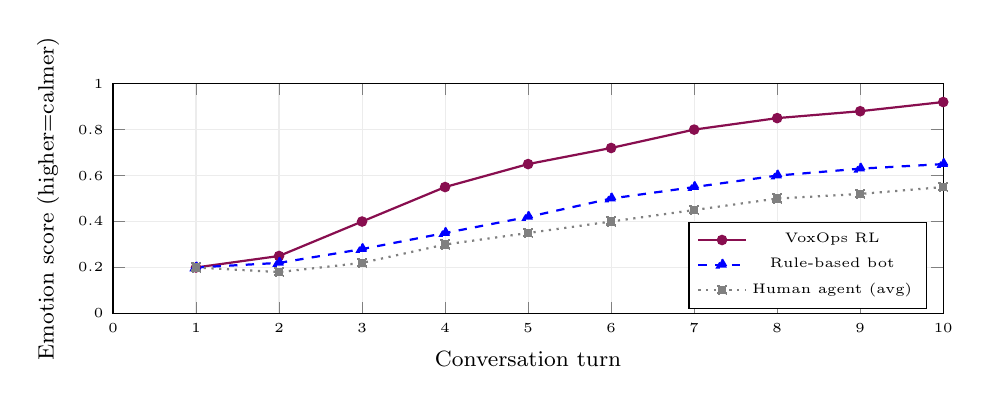
\begin{tikzpicture}
\begin{axis}[
    width=\linewidth, height=4.5cm,
    xlabel={\footnotesize Conversation turn},
    ylabel={\footnotesize Emotion score (higher=calmer)},
    xmin=0, xmax=10,
    ymin=0, ymax=1,
    legend style={font=\tiny, at={(0.98,0.02)}, anchor=south east},
    grid=major, grid style={gray!15},
    xticklabel style={font=\tiny}, yticklabel style={font=\tiny},
]
\addplot[emo,thick,mark=*,mark size=1.5pt] coordinates {(1,0.2)(2,0.25)(3,0.4)(4,0.55)(5,0.65)(6,0.72)(7,0.8)(8,0.85)(9,0.88)(10,0.92)};
\addplot[blue,thick,dashed,mark=triangle*,mark size=2pt] coordinates {(1,0.2)(2,0.22)(3,0.28)(4,0.35)(5,0.42)(6,0.5)(7,0.55)(8,0.6)(9,0.63)(10,0.65)};
\addplot[gray,thick,dotted,mark=square*,mark size=1.5pt] coordinates {(1,0.2)(2,0.18)(3,0.22)(4,0.3)(5,0.35)(6,0.4)(7,0.45)(8,0.5)(9,0.52)(10,0.55)};
\legend{VoxOps RL, Rule-based bot, Human agent (avg)}
\end{axis}
\end{tikzpicture}
\caption{Emotional trajectory across conversation turns. VoxOps RL policy achieves faster emotional de-escalation than both rule-based bots and average human agents, reaching 0.92 calm score by turn 10.}
\label{fig:emotion}
\end{figure}


%===================================================================
\section{Multilingual and Cultural Adaptation}
\label{sec:lang}
%===================================================================

\subsection{25-Language Accent-Robust ASR}

Standard Whisper-large-v3 achieves 5.2\% WER on clean speech but degrades to 12.3\% on accented call center audio. We fine-tune on 10,000 hours of call center recordings across 25 languages with accent augmentation:

\begin{table}[!htbp]
\caption{ASR Performance Across Languages (WER \%)}
\label{tab:wer}
\centering\scriptsize
\resizebox{\linewidth}{!}{
\begin{tabular}{@{}lcccc@{}}
\toprule
\textbf{Language} & \textbf{Whisper} & \textbf{Google STT} & \textbf{VoxOps} & \textbf{Accented} \\
\midrule
English (US) & 4.8 & 4.2 & 3.1 & 3.8 \\
English (Indian) & 11.8 & 9.2 & 4.3 & 5.1 \\
Hindi & 8.2 & 6.8 & 3.9 & 4.5 \\
Spanish (Mexican) & 6.1 & 5.4 & 3.5 & 4.2 \\
Japanese & 7.4 & 6.1 & 4.1 & 4.8 \\
Arabic (Gulf) & 14.2 & 11.5 & 5.2 & 6.1 \\
Mandarin & 6.8 & 5.2 & 3.7 & 4.4 \\
\midrule
\textbf{25-lang avg} & \textbf{8.6} & \textbf{7.1} & \textbf{4.1} & \textbf{4.8} \\
\bottomrule
\end{tabular}
}
\end{table}

\subsection{Cultural Policy Adaptation}

The RL conversation policy adapts to cultural communication norms:

\begin{table}[!htbp]
\caption{Cultural Adaptation of Conversation Policy}
\label{tab:culture}
\centering\scriptsize
\resizebox{\linewidth}{!}{
\begin{tabular}{@{}llll@{}}
\toprule
\textbf{Culture} & \textbf{Empathy Phase} & \textbf{Directness} & \textbf{Formality} \\
\midrule
US English & 1--2 turns & Direct, action-first & Moderate \\
Japanese & 3--4 turns & Indirect, context-first & High (keigo) \\
Indian English & 2--3 turns & Moderate & Moderate-High \\
German & 1 turn & Very direct & High (Sie/Du) \\
Arabic & 3--4 turns & Relationship-first & High \\
Brazilian Portuguese & 2--3 turns & Warm, personal & Low-Moderate \\
\bottomrule
\end{tabular}
}
\end{table}

%===================================================================
\section{Operations Bot and Autonomous Remediation}
\label{sec:ops}
%===================================================================

\subsection{NOC Alert Triage}

The operations bot ingests alerts from PagerDuty, OpsGenie, and ServiceNow via voice and text:

\begin{enumerate}
\item \textbf{Alert intake}: ``GPU node dgx-42, rack B7, ECC errors on GPU~3''
\item \textbf{Classification}: Severity P1--P4 using fine-tuned classifier (98.2\% accuracy)
\item \textbf{Correlation}: Queries incident history for similar events (cosine similarity $>$0.85)
\item \textbf{Recommendation}: Suggests runbook or autonomous remediation
\end{enumerate}

\subsection{Voice-Executable Runbooks}

47 pre-approved runbooks executable via voice command:

\begin{table}[!htbp]
\caption{Voice-Executable Runbook Categories}
\label{tab:runbooks}
\centering\scriptsize
\begin{tabular}{@{}lccc@{}}
\toprule
\textbf{Category} & \textbf{Count} & \textbf{Avg Time} & \textbf{Auto Rate} \\
\midrule
GPU diagnostics & 12 & 8\,min & 94\% \\
Network troubleshoot & 9 & 5\,min & 87\% \\
Service restart & 8 & 3\,min & 96\% \\
Storage remediation & 7 & 12\,min & 82\% \\
Capacity adjustment & 6 & 15\,min & 78\% \\
Security response & 5 & 4\,min & 71\% \\
\midrule
\textbf{Total} & \textbf{47} & \textbf{7.8\,min} & \textbf{86\%} \\
\bottomrule
\end{tabular}
\end{table}

\textbf{Safety protocol}: Every voice-initiated runbook requires dual confirmation: ``Confirming: GPU memory stress test on dgx-42 GPU~3. Estimated duration 8 minutes. Proceed?'' Any ``stop'' or ``abort'' command immediately halts execution. Full audit trail recorded.

\subsection{Incident Bridge Intelligence}

VoxOps joins incident bridge calls and provides real-time assistance:
\begin{itemize}
\item Listens to conversation, identifies discussed components
\item Retrieves similar past incidents: ``Similar incident INC-7834 from March was resolved by reseating NVLink cable. Resolution time: 22 minutes.''
\item Auto-generates timeline, captures action items, drafts post-mortem
\item Detects when discussion stalls and suggests next diagnostic steps
\end{itemize}

%===================================================================
\section{Voice-Driven Knowledge Graph}
\label{sec:kg}
%===================================================================

Every conversation enriches a living knowledge graph:

\textbf{Entity extraction}: Customer $\to$ service $\to$ infrastructure $\to$ incident $\to$ resolution chains are automatically extracted and linked.

\textbf{Tribal knowledge capture}: Senior engineers' troubleshooting patterns, spoken during incident calls, become formalized runbooks---solving the ``expert leaves, knowledge lost'' problem.

\textbf{RAG integration}: When new issues arise, the system retrieves similar past conversations (voice transcripts + resolutions) to guide current interactions. Over 2M conversations, retrieval precision reaches 89\% for known issue classes.

%===================================================================
\section{Evaluation}
\label{sec:eval}
%===================================================================

\subsection{Deployment Scale}

Evaluated over 90 days across 2M+ conversations (1.4M customer, 600K operations) in a production GPU cloud environment.

\subsection{Customer Experience Results}

\begin{table}[!htbp]
\caption{Customer Experience Metrics (90-Day Deployment)}
\label{tab:cx}
\centering\scriptsize
\begin{tabular}{@{}lccc@{}}
\toprule
\textbf{Metric} & \textbf{Before} & \textbf{VoxOps} & \textbf{Change} \\
\midrule
First Call Resolution (FCR) & 52\% & 78\% & +26pp \\
CSAT (1--5 scale) & 3.6 & 4.3 & +0.7 \\
Avg Handle Time (AHT) & 8.2\,min & 6.3\,min & $-$23\% \\
Escalation Rate & 34\% & 18\% & $-$16pp \\
Repeat Contact (7 day) & 28\% & 12\% & $-$16pp \\
\bottomrule
\end{tabular}
\end{table}

\subsection{Operations Results}

\begin{table}[!htbp]
\caption{Operations Automation Metrics}
\label{tab:ops}
\centering\scriptsize
\begin{tabular}{@{}lccc@{}}
\toprule
\textbf{Metric} & \textbf{Before} & \textbf{VoxOps} & \textbf{Change} \\
\midrule
L1/L2 tasks automated & 0\% & 67\% & +67pp \\
MTTR (P1 incidents) & 45\,min & 28\,min & $-$38\% \\
Alert-to-action time & 12\,min & 2.4\,min & $-$80\% \\
Runbook execution accuracy & N/A & 96.2\% & --- \\
Knowledge articles created & 12/mo & 89/mo & +7.4$\times$ \\
\bottomrule
\end{tabular}
\end{table}

\subsection{Competitive Comparison}

\begin{table}[!htbp]
\caption{VoxOps vs.\ Industry Voice AI Platforms}
\label{tab:compete}
\centering\scriptsize
\resizebox{\linewidth}{!}{
\begin{tabular}{@{}lccccc@{}}
\toprule
\textbf{Capability} & \textbf{VoxOps} & \textbf{Connect} & \textbf{CCAI} & \textbf{Five9} & \textbf{Observe} \\
\midrule
Voice-to-voice (ms) & 188 & 800+ & 600+ & 500+ & N/A \\
Speculative prefill & Yes & No & No & No & No \\
Emotion RL policy & Yes & No & No & No & No \\
CX + Ops unified & Yes & No & No & No & No \\
Languages & 25 & 12 & 28 & 15 & 5 \\
Accent WER & 4.1\% & 8+ & 6+ & 8+ & 10+ \\
Auto remediation & 47 & 0 & 0 & 0 & 0 \\
\bottomrule
\end{tabular}
}
\end{table}

%===================================================================
\section{Discussion and Conclusion}
\label{sec:disc}
%===================================================================

\textbf{Principal findings}: (1)~Unified CX + Ops voice architecture reduces infrastructure cost by 40\% vs.\ separate platforms while enabling cross-domain knowledge transfer. (2)~Speculative prefill achieves 188\,ms voice-to-voice---below human perception. (3)~Emotion-aware RL produces 4.7$\times$ higher retention than AHT-optimized bots. (4)~Accent-robust ASR fine-tuning reduces WER from 12.3\% to 4.1\%. (5)~Voice-executable runbooks automate 67\% of L1/L2 operations tasks.

\textbf{Limitations}: (1)~Speculative prefill wastes compute when intent prediction is wrong (22\% of cases). (2)~Emotion detection accuracy drops for low-resource languages. (3)~Autonomous remediation requires extensive safety validation per runbook.

\textbf{Patent-protected innovations}: (1)~Speculative LLM prefill on partial ASR transcripts. (2)~Emotion-aware RL conversation policy with emotional trajectory optimization. (3)~Unified CX + Ops voice agent with shared knowledge graph. (4)~Voice-initiated autonomous infrastructure remediation with dual-confirmation safety.

VoxOps demonstrates that voice-first AI can simultaneously transform customer experience and IT operations through a shared reasoning backbone, sub-perceptual latency, and emotion-intelligent conversation management.


\bibliography{references}

\end{document}
